The optimized parameters  for the SPL and BPL models are summarized in Table~\ref{tb:bestparams}. 
The best-fit $\gamma$-ray spectra from the two models
compared to the thin-target Earth's limb measurement by the LAT are illustrated
in Figure~\ref{fig:gamma-flux}, showing very similar results for both models.
Since the proton-to-$\gamma$ energy conversion factor is roughly 0.17 for broad
and smooth spectra [10], our inferred CR proton spectra are valid between 60 - 2000 GV
in rigidity as shown in comparison with measurements by other instruments in Figure~\ref{fig:proton-flux}.
Note that the normalizations of our work in Figure~\ref{fig:proton-flux} are scaled
by fitting to AMS-02 data between 100~-~2000~GV.
% eye to approximately match PAMELA data.
% has shown in Table~\ref{tb:bestparams}.
% According to figure \ref{fig:gamma-flux}, secondary $\gamma$-ray product
% from both SPL and BPL model yield a similar product via hadronic collision
% in the atmosphere. In order to validate the indirect measurement of CR proton,
% comparing with a real observations is mandatory which has shown
% in figure \ref{fig:proton-flux}. The normalization of this work is
% fitted PAMELA data to roughly scale the incident proton spectrum.

\begin{figure}[h!]
    \centering
    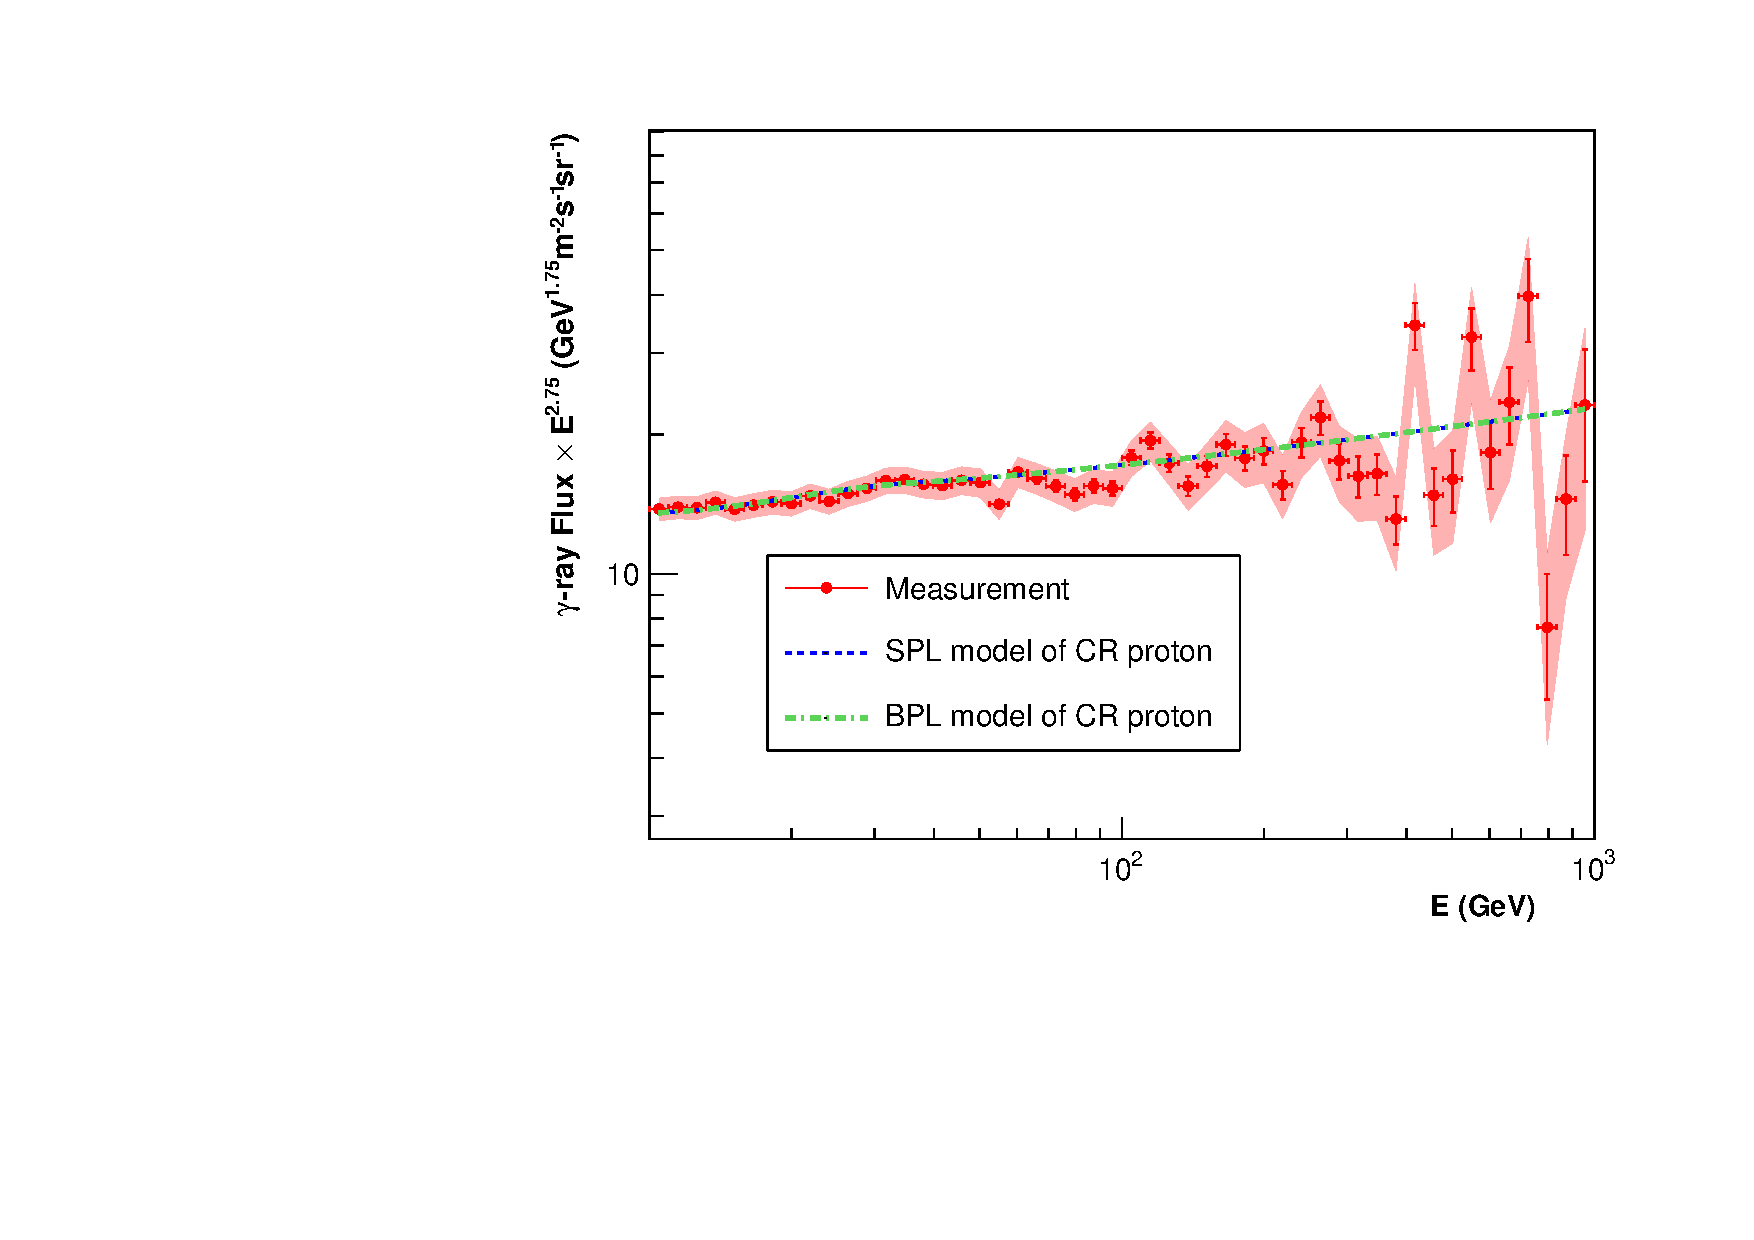
\includegraphics[width=0.7\textwidth]{img/fitted_result}
    % \caption{Measured $\gamma$-ray flux and the product from incident CRs}
    \caption{
        The $\gamma$-ray spectra calculated from the SPL (blue)
        and BPL (green) models of CR proton which best fit with the measured Earth's
        $\gamma$-ray spectrum in the thin-target regime (red).
    }
    \label{fig:gamma-flux}
\end{figure}



\begin{center}
\begin{table}[h]
\centering
\caption{Best-fit CR proton spectral parameters} 
\label{tb:bestparams}
\begin{tabular}{@{}l*{15}{l}}
\br
CR proton model&Index 1&Index 2&$E_\text{break}$ (GeV)\\
\mr
SPL&2.70&-&-\\
BPL&2.86&2.63&333\\
\br
\end{tabular}
\end{table}
\end{center}


\begin{figure}[h!]
    \centering
    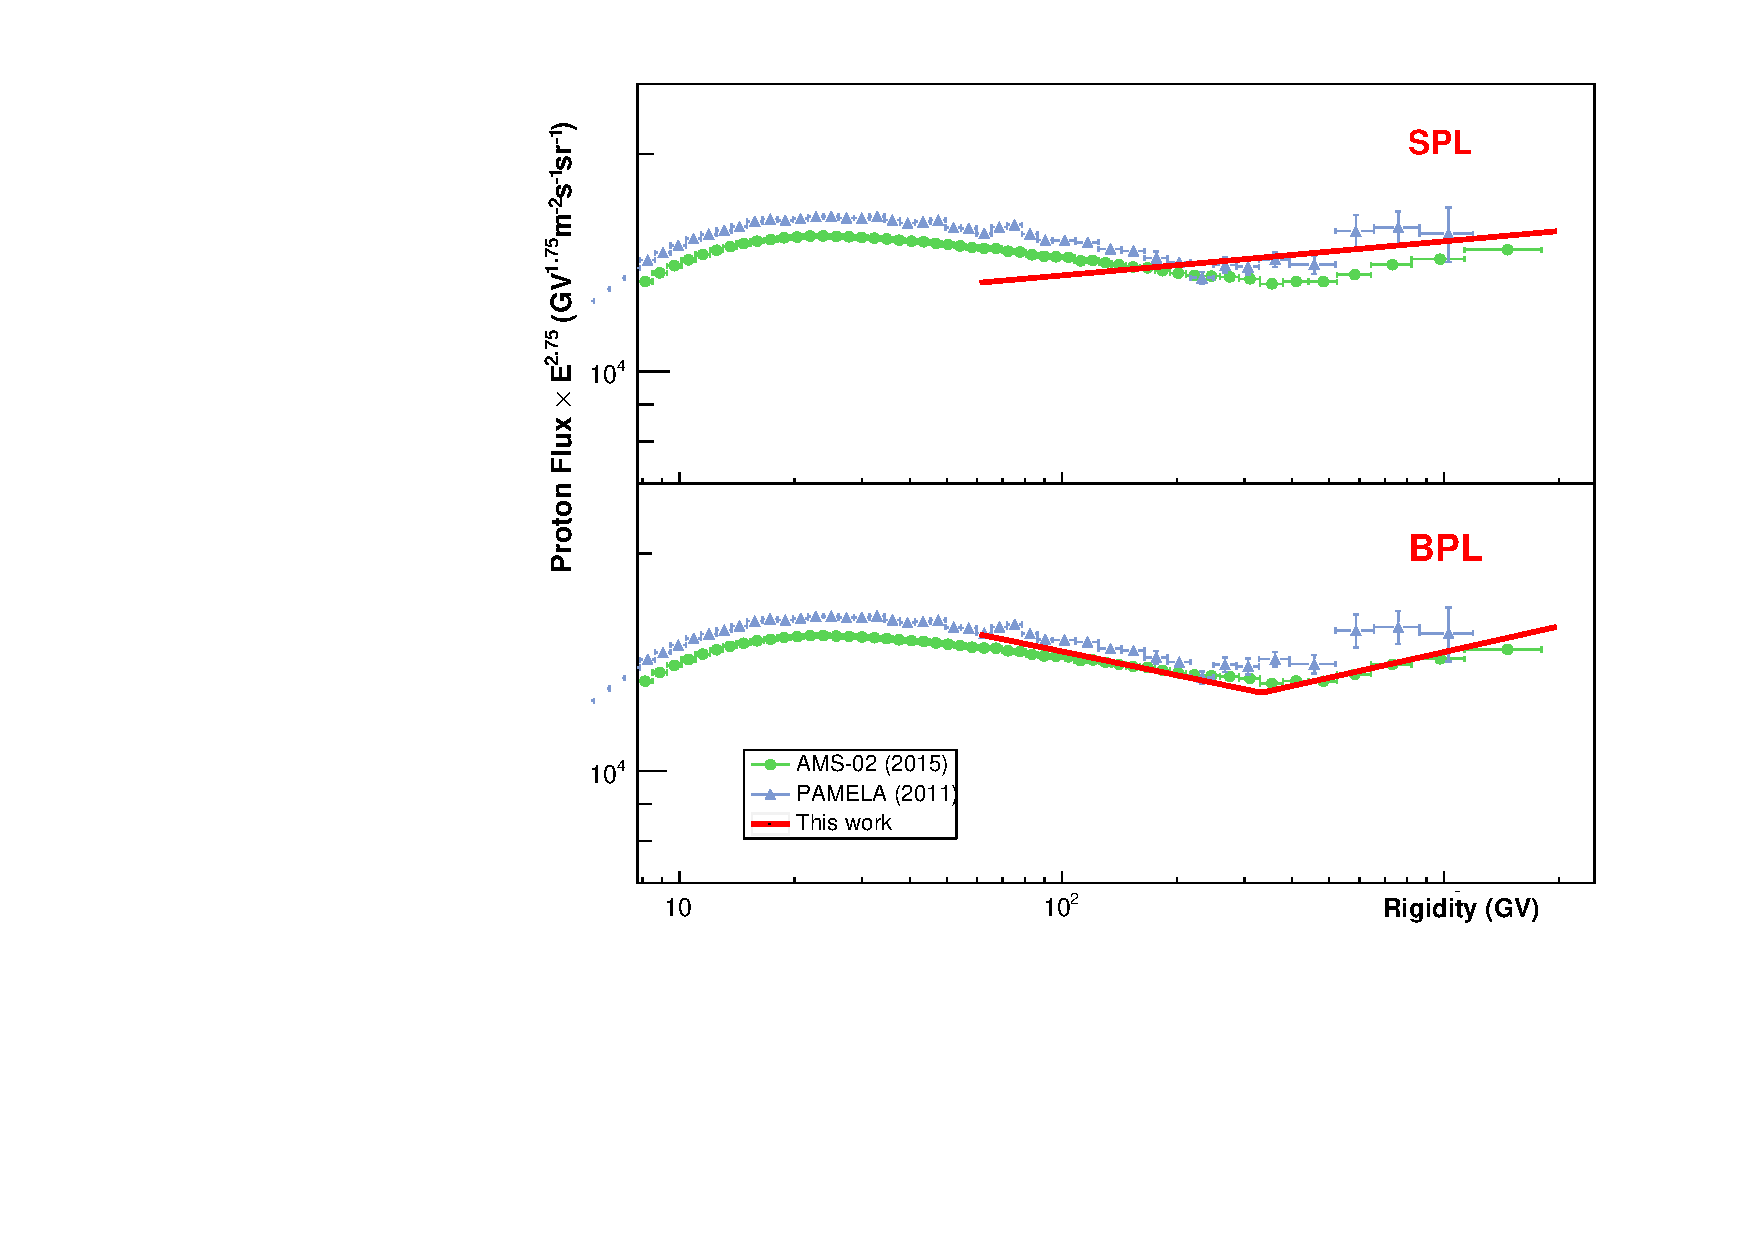
\includegraphics[width=0.8\textwidth]{img/ProtonSpectrumModelMeasurement.pdf}
    % \caption{Best fitted proton CRs versus real observations}
    \caption{Best-fit CR proton spectrum from this work (red) compared to the measurements by AMS-02 (blue) and PAMELA (green).}
    \label{fig:proton-flux}
\end{figure}

